\documentclass[a4paper,10pt,oneside]{article}
\usepackage[polutonikogreek,italian]{babel}
\usepackage[utf8x]{inputenc}
\usepackage{amsmath}
\usepackage{amsthm}
\usepackage{amssymb}
\usepackage{amscd}
\usepackage{graphicx}
\usepackage{float}
\usepackage{array}
\usepackage{rotating}
\usepackage[small]{caption}
\usepackage{lscape}
\usepackage{fancybox}
\usepackage{booktabs}
\usepackage[noanswer]{exercise}
\parindent0ex
\renewcommand{\fboxsep}{0.4cm}
\usepackage{hyperref}
\renewcommand{\textfraction}{0.05}
\renewcommand{\topfraction}{0.95}
\renewcommand{\bottomfraction}{0.95}
\renewcommand{\floatpagefraction}{0.35}
\renewcommand{\ExerciseName}{Esercizio}
\renewcommand{\ExerciseListName}{Es}
\setcounter{totalnumber}{5}
\restylefloat{figure}
\begin{document}
\section*{Il lavoro della forza elastica}


Ricordiamo che abbiamo definito la forza elastica come:
\begin{equation}
 \mathbf{F}=-k\mathbf{x}
\end{equation}
questa legge può essere applicata a delle molle reali per un  ampio intervallo di valori di $|\mathbf{x}|$.
Il vettore $\mathbf{x}$ rappresenta lo spostamento della molla dalla sua posizione di riposo e $k$ la costante elastica della molla.
Calcoliamo ora il lavoro fatto dalla molla quando questa viene allungata di una quantità $\mathbf{x}$ tramite l'applicazione di una forza esterna (es la molla viene allungata dall'osservatore) come in figura [\ref{fig:molla_allungata}]

\begin{figure}[H]
 \centering
 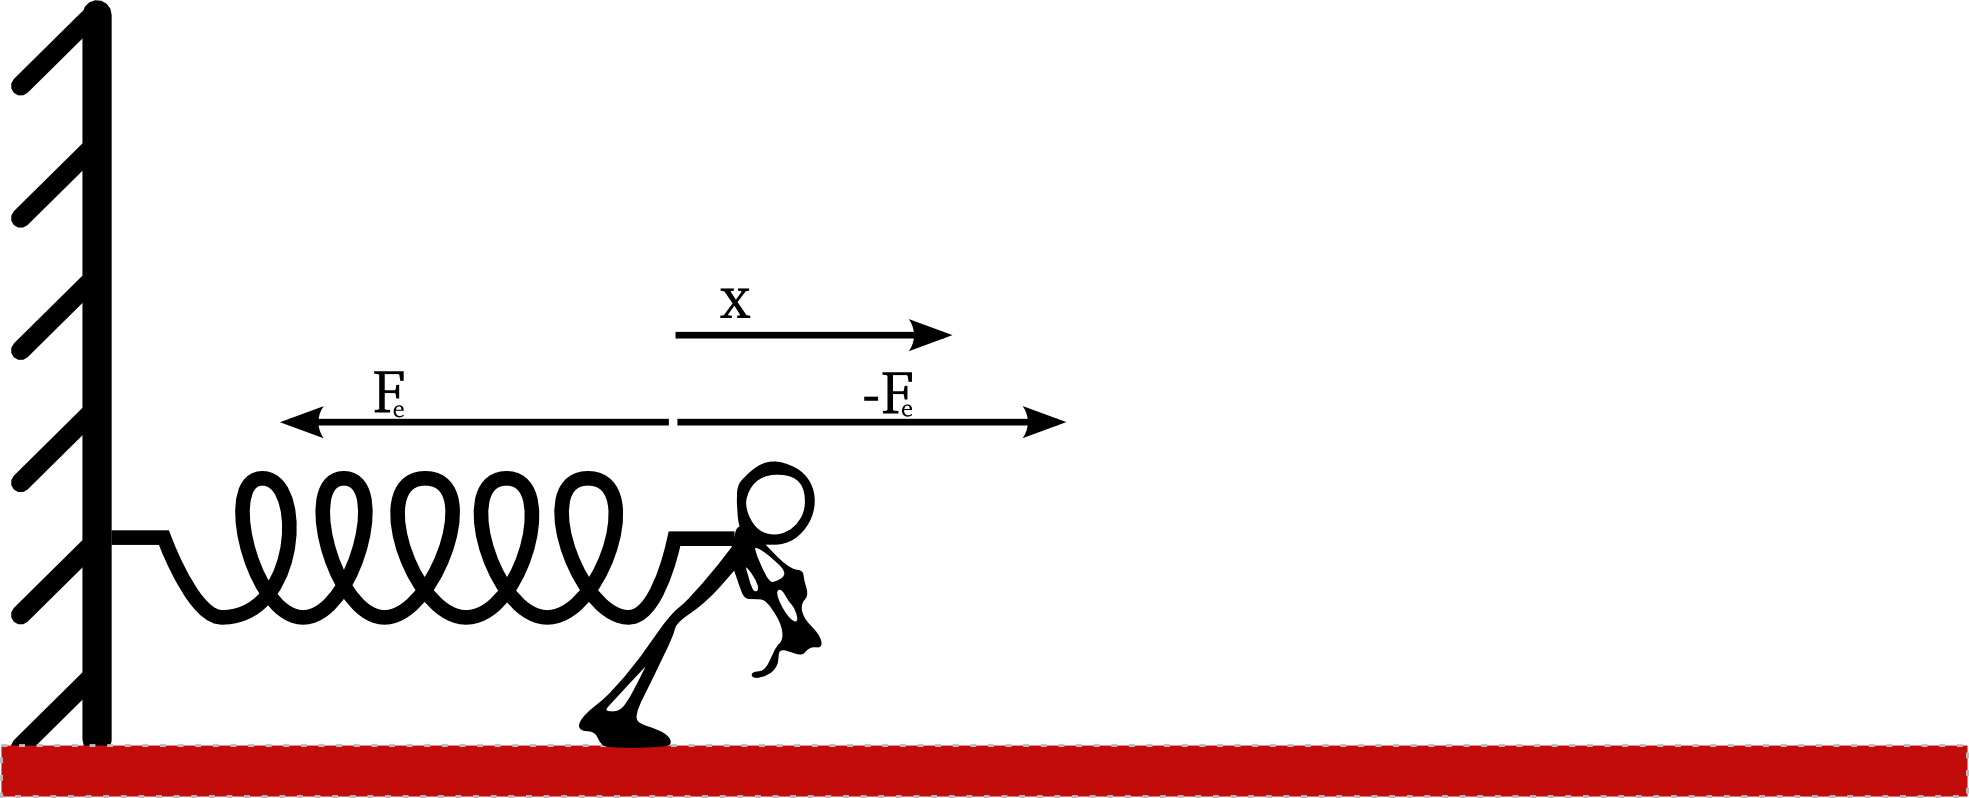
\includegraphics[width=\textwidth]{./immagini/lavoro_molla1.png}
 % lavoro_molla1.png: 1969x798 pixel, 300dpi, 16.67x6.76 cm, bb=0 0 473 192
 \caption{La molla viene allungata da una forza in ogni istante uguale alla forza elastica $F_e$, il processo è infinitamente lento}
 \label{fig:molla_allungata}
\end{figure}

La forza elastica e lo spostamento $\mathbf{x}$ hanno verso opposto quindi i due vettori formano tra loro un angolo pari a $\pi$ radianti. Nel caso in cui la forza sia costante durante lo spostamento abbiamo definito il lavoro come:
\begin{equation}
 L=\mathbf{F}\cdot \mathbf{S}
\end{equation}
nel caso della molla la forza non è però costante durante lo spostamento, per calcolare il lavoro dovremo quindi utilizzare la strategia seguita durante il calcolo della potenza per velocità non costanti.
Immaginiamo di suddividere l'intervallo di lunghezza $|\mathbf{x}|$ in tanti segmenti uguali di lunghezza $\Delta x$ considerando costante la forza elastica all'interno di ognuno di questi possiamo dire che il modulo della forza elastica nell'ennesimo intervallino sarà:
\begin{equation}
 F_n=kn\Delta x
\end{equation}
mentre il lavoro fatto da questa forza costante all'interno di ogni intervallino sarà:
\begin{equation}
L_n=-nk(\Delta x)^2
\end{equation}
dove il segno meno è dovuto al fatto che la forza elastica e lo spostamento hanno versi opposti.
Una approssimazione del lavoro totale sarà data dalla somma dei lavori delle forze costanti all'interno di ognuno degli intervallini:
\begin{equation}
 L\sim L_1+L_2+L_3+\ldots+L_N
\end{equation}
Se riportiamo in un grafico, in ordinata il valore della forza per il coseno dell'angolo compreso e in ascissa lo spostamento otteniamo il grafico di figura [\ref{fig:lavoro_molla_negativo}]
\begin{figure}[H]
 \centering
 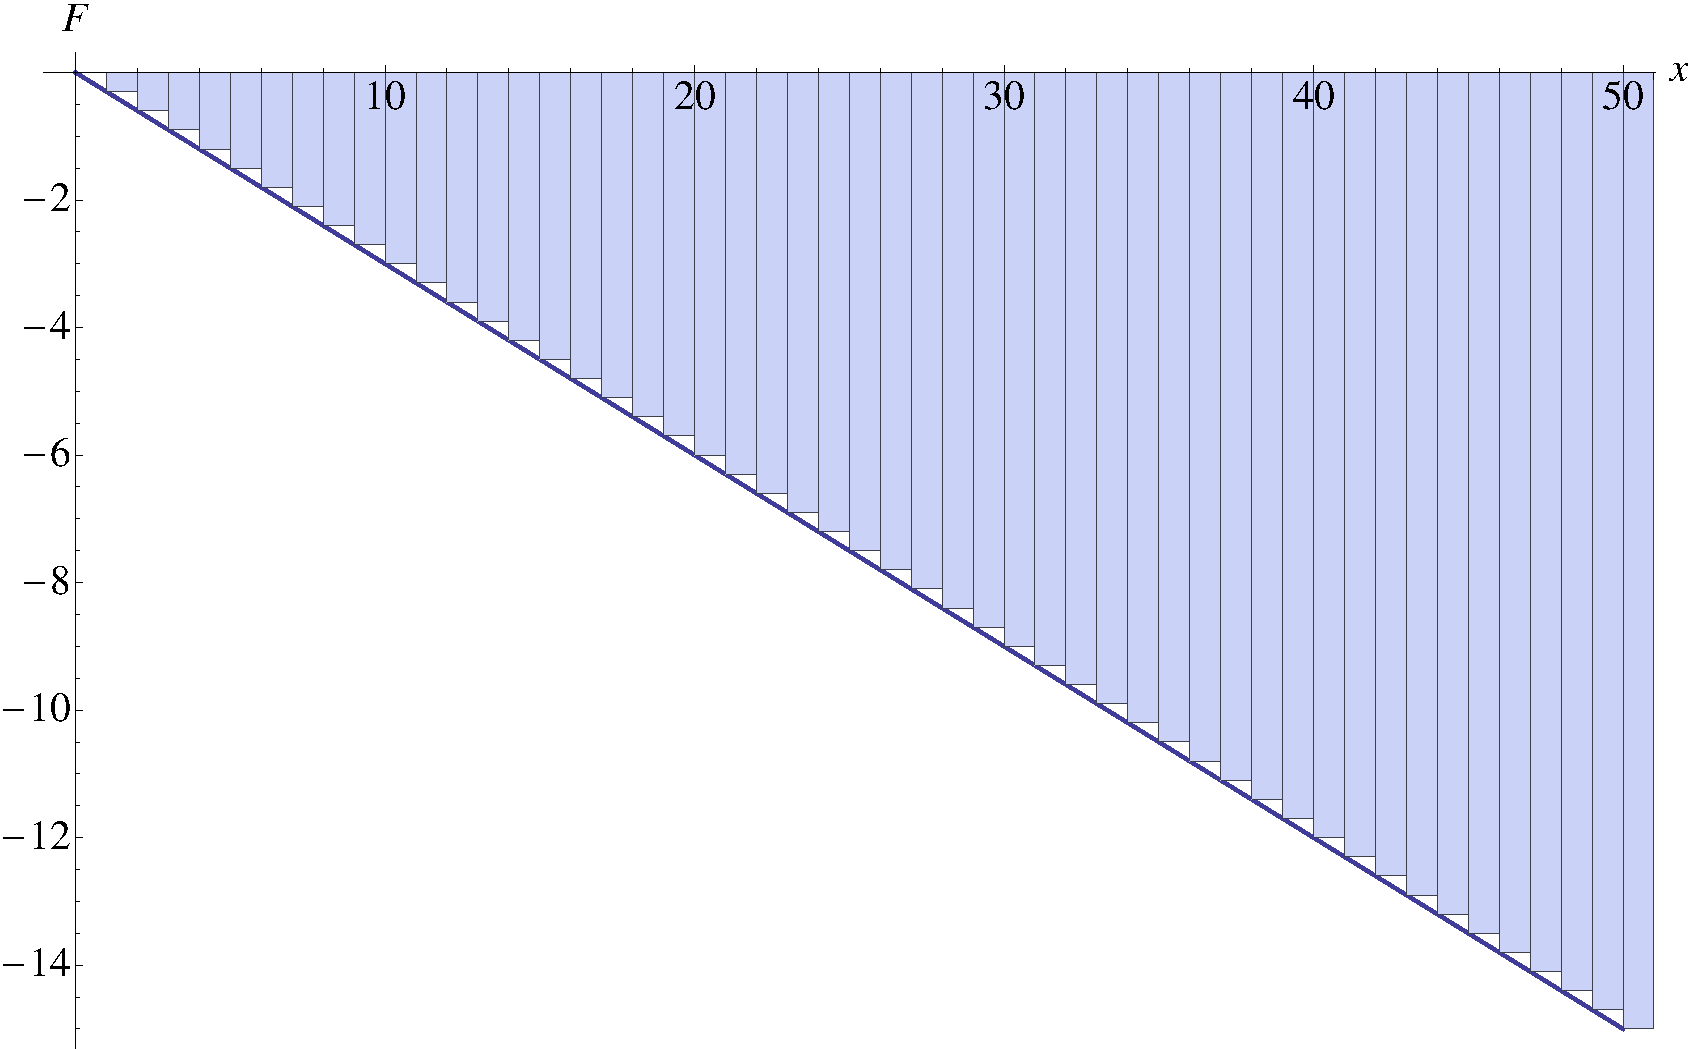
\includegraphics[width=\textwidth]{./immagini/lavoro_molla_negativo.pdf}
 % lavoro_molla_negativo.pdf: 810x503 pixel, 72dpi, 28.58x17.74 cm, bb=0 0 810 503
 \caption{Il lavoro eseguito dalla molla è negativo, lo spostamento  e la forza elastica hanno versi opposti}
 \label{fig:lavoro_molla_negativo}
\end{figure}
vediamo che tanto più piccoli sono gli intervalli in cui abbiamo diviso lo spostamento tanto più la somma delle superfici dei rettangoli si avvicina alla superficie del triangolo avente come base lo spostamento e come altezza la forza nella posizione estrema. Al tendere del numero di intervalli all'infinito la somma delle aree  dei rettangoli diverrà pari all'area del triangolo, potreom quindi scrivere:
\begin{equation}
 L_m=-\frac 1 2 kx^2
\end{equation}
il segno meno è sempre dovuto al fatto che lo spostamento e la forza hanno versi opposti. Il lavoro svolto dalla persona che sta allungando la molla sarà invece positivo dato che la forza di allungamento ha verso opposto alla forza elastica e quindi uguale allo spostamento:
\begin{equation}
L_p=\frac 1 2 kx^2
\end{equation}

la somma dei lavori è nulla dato che la forza totale agente in questo caso è pari a zero. I rettangolini che otteniamo in questo caso avranno area positiva e il grafico sarà quello di figura [\ref{fig:lavoro_molla_approssimazione}]

\begin{figure}[H]

 \centering
 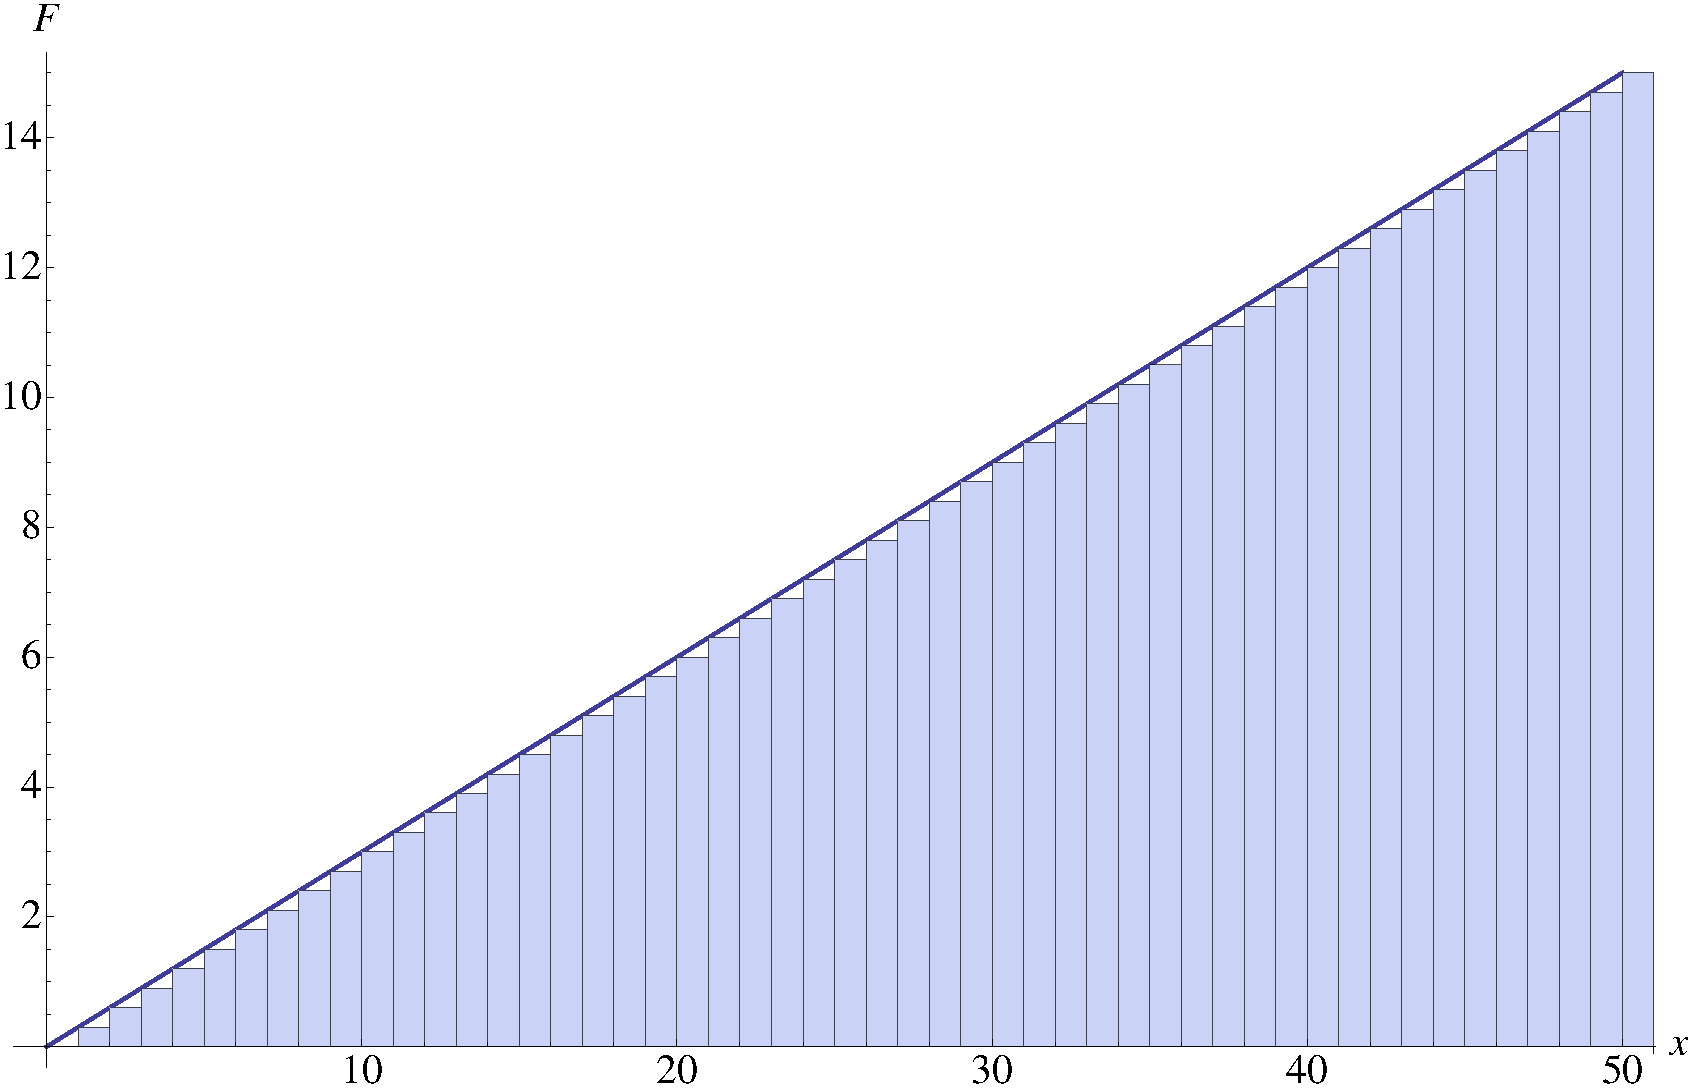
\includegraphics[width=\textwidth]{./immagini/lavoro_molla.pdf}
 % lavoro_molla.pdf: 810x524 pixel, 72dpi, 28.58x18.49 cm, bb=0 0 810 524
\caption{Se lo spostamento e la forza hanno verso concorde il lavoro è positivo}\label{fig:lavoro_molla_approssimazione}
\end{figure}

Se invece di allungare la molla la comprimiamo il segno e il modulo dei lavori non varieranno infatti lo spostamento avrà sempre il verso della forza premente mentre la forza elastica verso opposto:
\begin{figure}[H]
 \centering
 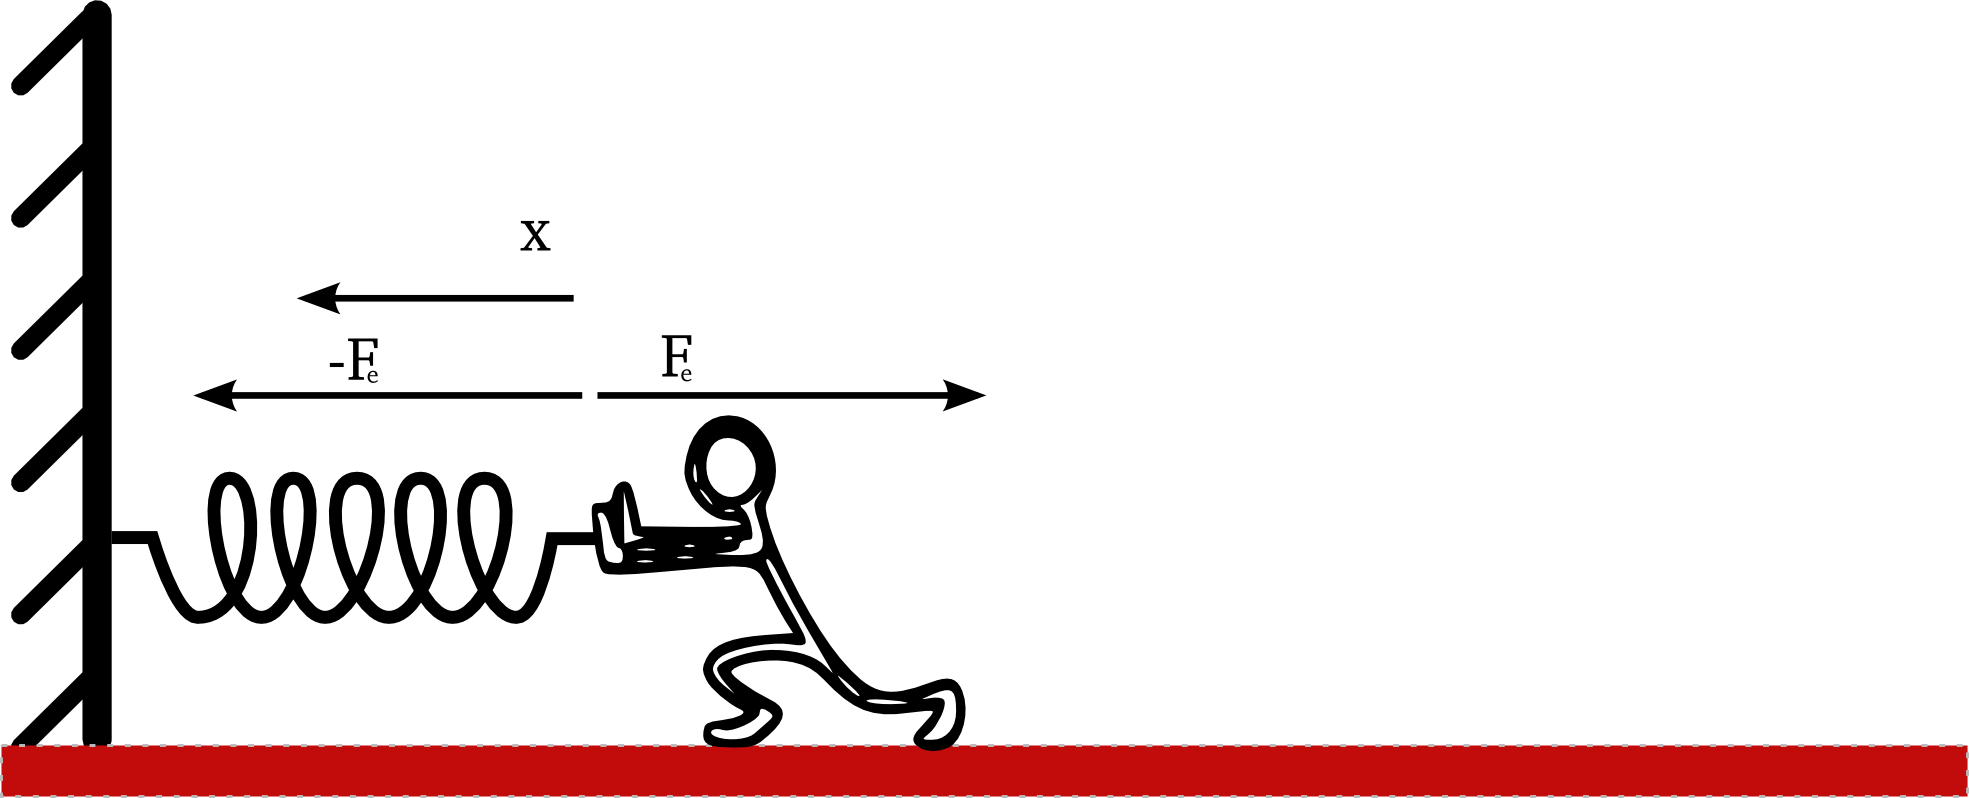
\includegraphics[width=\textwidth]{./immagini/lavoro_molla2.png}
 % lavoro_molla2.png: 1969x798 pixel, 300dpi, 16.67x6.76 cm, bb=0 0 473 192
 \caption{La forza elastica ha verso opposto allo spostamento anche durante una compressione}
 \label{fig:compressione_molla}
\end{figure}




\end{document}
